\chapter{The multi agent system}
\label{ch:multiagentsystem}

This chapter gives an overview of which parts is the MAS composed, how its internal parts work, which communication schemes it uses and how it works.

JADE uses a peculiar system of agents and behaviors, agents represent a static class that keeps all the information stored but doesn't do anything by itself, that's the behaviors job. Behaviors are like scheduled actions for that specific class, such as moving the car this time unit or drawing the new added cars in the GUI.

It is important for behaviors not take a lot of time, since that is the way to sharing computing time between resources, you execute your behavior and \textit{go to sleep} while other behaviors are executed. This makes for a really fast and efficient way of sharing resources if used correctly.

In this MAS, every behavior takes one Tick (it represent a second on the simulator timescale) to finish, then depending on its nature it will be repeated until an ending condition is reached.

\section{Multi agent system models overview}

In this section an overview of the different models that the system uses will be done, as well as a brief definition of the implemented classes.

\subsection{Agent model}

This subsection details the JADE agents used by the system.

\subsubsection{Car agent}

This agent represents a mobile vehicle with a set maximum speed that moves from a starting point to a destination via valid paths. The route that follows is determined by the type of routing algorithm chosen.

\subsubsection{Event manager agent}

This agent reads all the events from a file and executes them at specific points in time, this helps the system to have a deterministic behavior if anyone wants to redo the experiments.

\subsubsection{Interface agent}

This agent is keeps all the information about the GUI and is the one that has to keep all its information updated. It also reads the user inputs (such as changing the timescale).

\subsubsection{Segment agent}

This agent represents a road side unit on one segment of the network, that is the connection between two intersections. The road side unit covers the full extent of the segment. All car agents register on it when entering and deregister when leaving, he is in charge of communicating the GUI the position of its car agents, so that the number of messages is reduced (from one message per car to one message per segment).

\subsubsection{Time keeper agent}

This agent keeps the simulation synchronized between all agents, this makes keeping track of time and making scheduled events possible. This is the key to make all the cars move at the same time and, schedule events at a certain moment of the day (such as 12:00).

\subsection{Behavior model}

This subsection details the behaviors used by the system.

\subsubsection{Car behavior}

This behavior is used by the Car agent and calculates the next graphical position of the car. It also registers and deregisters the car from the segments. Registering is done when the car enters in a new segment and deregistering is done when the car exits a segment.

In every tick it moves and registers or deregisters of the segment if needed, this is a cyclic behavior that ends when the car reaches its destination.

\subsubsection{Event manager behavior}

This behavior is used by the Event manager agent. It executes the events that has in memory that have previously been read by its agent, if it is the time to execute that event it sends the instructions to the interested party. It also formats the time displayed in the GUI so that it is human readable.

In every tick it sends all the necessary messages if a event is executed, it also sends a message to update the time. This is a cyclic behavior that ends when the simulation ends.

\subsubsection{Interface add car behavior}

This behavior is used by the Interface agent, it receives the instructions to create a new car (from the manager behavior) and creates the graphical representation of it and keeps it updated.

In every tick it checks if a new car has to be added. This is a cyclic behavior that ends when the simulation ends.

\subsubsection{Interface draw behavior}

This behavior is used by the Interface agent (agents can have more than one behavior) and it updates all the parts of the GUI. It updates all the cars position on the GUI, adds new cars to the GUI, deletes cars that have finished from the GUI and updates the time and the number of cars on the GUI.

In every tick it checks whether he has to update the any part of the GUI or not (usually it has to update all the cars position since they move every tick). This is a cyclic behavior that ends when the simulation ends.

\subsubsection{Segment listen behavior}

This behavior is used by the Segment agent and listens to messages from cars to register or deregister, or to update their position. It also listens for messages from the Event manager in case it needs to change its service level.

In every tick it checks for messages from cars or events and updates its lists of registered cars. This is a cyclic behavior that ends when the simulation ends.

\subsubsection{Segment send to draw behavior}

This behavior is used by the Segment agent and sends the information about the cars that are registered on it to the Interface agent so it updates the car positions.

In every tick if there are any cars on it, it sends their information to the interface agent. This is a cyclic behavior that ends when the simulation ends.

\subsection{Representation model}

This subsection describes the classes that the system uses to model the road network.

\subsubsection{Intersection}

This class represents an intersection, that is a point on the map where one or more segments end or start. It is only possible for a car to change between segments here.

\subsubsection{Segment}

This class represents the connection between two intersections. Each segment has a origin and an end, it also keeps all the important information such as maximum speed, number of tracks and density. This class also has a list of steps that contain the information for its graphical representation.

\begin{figure}[!ht]
  \centering
  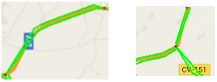
\includegraphics[scale=2]{images/intersectionSegment.png} 
  \caption{An example of segment and intersection}
\end{figure}

\subsubsection{Step}

This class is used to represent a line in the canvas where the graphical map is drawn, it contains the $x$ and $y$ coordinates for the initial and ending point of that line, segments are usually made up of more than one step so its graphical representation is real life like.

\subsubsection{Path}

This class is used to keep the segments and steps that a car has to follow to get from its origin to its destination, this path can be dynamically computed depending on the algorithm of choice.

\subsubsection{Map}

This class represents the whole road network, it reads the data from file and instances all the necessary classes to build the directed graph, it also instances the segment agents. It provides many methods to work with the graph.

\subsection{CanvasWorld}

This class contains all the information that is needed to draw the GUI, it also contains an API that allows the Interface agent to modify its contents.

\subsection{Main}

This is the class that is called when the program is started it spawns the required JADE services. It also provides a few configuration options that are worth mentioning:

\begin{itemize}
\item \textbf{tickLength}: This parameter is used when the application is used in headless mode, that is without spawning the GUI, which is very useful for servers. This overwrites the default tickLength that is usually set by the user via a slider in the GUI. \textit{Default}: 1L
\item \textbf{startingTick}: This is the tick at which the application starts, because this tick represents one simulation second you can do something like $7*3600 + 30*60$ to make it start at 7:30 am. \textit{Default}: $7*3600 + 59*60$
\item \textbf{finishingTick}: This is the tick at which the simulation will end. \textit{Default}: $24*3600$
\item \textbf{numberOfCars}: This parameter allows the user to put a certain number of smartcars at the beginning of the simulation, this is very useful for stress tests. \textit{Default}: 0
\item \textbf{drawGUI}: This parameter allows running the application in headless mode. \textit{Default}: true
\item \textbf{startRMA}: This parameter allows the control of starting the JADE Remote Agent Management, which is an interface to an administration panel for the agents. \textit{Default}: false
\item \textbf{segmentLogging}: This parameter allows the control of the logging system. \textit{Default}: false
\item \textbf{loggingDirectory}: This parameter allows us to change where the log files will be stored. \textit{Default}: ""
\end{itemize}

\subsection{Search algorithms}

At the moment of writing this thesis, there are only three implemented algorithms. The system uses the Factory method programming pattern \cite{wikipedia_factory} so that if any researcher wants to add a new algorithm he or she can do it easily. The algorithms are further explained in Chapter \ref{ch:stateoftheart}.

\subsubsection{Shortest path algorithm}

This algorithms is an implementation of the Dijkstra's algorithm \cite{wikipedia_dijkstra} that looks for the shortest path on the graph. Cars using this algorithm always take the same path given the same origin and the same destination.

\subsubsection{Fastest path algorithm}

This algorithm is a modification of Dijkstra's that focuses on time rather than on distance, this algorithm searches for the longest time for a given segment knowing the maximum speed of the car and of that segment. This \textbf{does not} take into account the state of the traffic.

\subsubsection{Smartest path algorithm}

This algorithm is yet another modification of Dijkstra's algorithm, this algorithm focuses on minimizing the trip time and takes into account the current traffic, so that if there is a congestion on a path and the average speed is slower, it will change to a longer path whose total trip time is lower.

\subsection{Knowledge model}

This subsection describes the files that make up the knowledge model database

\subsubsection{Events}

A file of events is needed so the simulator can run them, the file should be in \textit{csv} format.

\begin{table}[H]
\centering
\begin{tabular}{|c|c|c|c|c|c|}
\hline 
\textbf{Type} & \textbf{Time} & \textbf{Origin} & \textbf{Ending} & \textbf{Maximum speed} & \textbf{Algorithm} \\ 
\hline 
newCar & 08:53 & I-CV10-08 & I-N340-07 & 86 & fastest \\ 
\hline 
newCar & 22:27 & I-AP7-01 & I-CV10-03 & 114 & shortest \\ 
\hline 
newCar & 11:07 & I-AP7-01 & I-CV10-04 & 86 & shortest \\ 
\hline 
newCar & 11:46 & I-CV10-04 & I-CS22-04 & 105 & smartest \\ 
\hline 
\end{tabular}
\caption{A few rows of the events.csv file}
\end{table}

A Python script to generate this file is also provided in the root of the project, called \emph{generateRandomEvents.py} which allows for an easy creation of test files.

\subsubsection{Map files}

This are the files where the Map class takes its data:

\begin{itemize}
\item \textbf{intersections}: A JSON file containing the information about the intersections and their position on the graphical map.
\item \textbf{segments}: A JSON file containing the information of the segments, including origin and destination, maximum speed, length, etc.
\item \textbf{steps}: A JSON file that contains the steps that make up a segment, remember that the steps are the graphical representation of the segment, whereas the segment does not have a representation by itself.
\end{itemize}

\subsubsection{Images}

There are also three images that are needed on this simulator:

\begin{itemize}
\item \textbf{icon.png}: That's the icon that will appear on the top left corner of the GUI.
\item \textbf{legend.png}: This is a legend of the simulator, it helps interpreting the data.
\item \textbf{red.png}: This is the image used to represent the road network, a Google Maps screenshot.
\end{itemize}

\section{Interaction model}

Due to the distributed nature of this simulator, all the communication between classes has to be done through messages. JADE allows us to set different kind of communication ontologies so classes know what type of arguments to expect and what to do with those arguments. We can see in Figure \ref{ontologyScheme} the different communication ontologies used between classes, this simulator uses quite a few. A brief description of them is done in Table \ref{ontologiesTable}.

\begin{table}[h]
\centering
\begin{adjustbox}{angle=90}    

\begin{tabularx}{\textheight}{|X|c|c|c|X|}
\hline 
\textbf{Name} & \textbf{From} & \textbf{To} & \textbf{Arguments} & \textbf{Description} \\ 
\hline 
logOntology & Event manager agent & Interface agent & String & Tells the interface agent which text to add to the log panel \\ 
\hline 
drawOntology & Segment agent & Interface agent & String & Sends the information about the cars that have to be drawn \\ 
\hline 
newCarOntology & Car agent & Interface agent & String & Adds a car for the first time \\ 
\hline 
changeTickLengthOntology & Interface agent & Timekeeper agent & Integer & Changes the ticklength on the simulation \\ 
\hline 
tickOntology & Timekeeper agent & Car, segment and Manager agents & Long & Tells everyone to compute an additional tick \\ 
\hline 
numberOfCarsOntology & Timekeeper agent & Interface agent & Integer & Tells the interface how many cars are running in the simulation \\ 
\hline 
carToSegmentOntology & Car agent & Segment agent & String & Tells the segment to register, deregister or update this car \\ 
\hline 
deleteCarOntology & Car agent & Interface agent & String & Tells the interface to delete that car \\ 
\hline 
updateTimeOntology & Event manager agent & Interface agent & String & Tells the interface to update the displayed clock \\ 
\hline 
eventManagerToSegmentOntology & Event manager agent & Segment agent & String & Tells a segment to change its service level \\ 
\hline 
\end{tabularx}
\end{adjustbox}
\caption{The complete list of ontologies}
\label{ontologiesTable}
\end{table}

\begin{figure}[!ht]
  \centering
  \includegraphics[scale=0.8]{images/ontologyScheme80.png} 
  \caption{Ontology communications scheme}
  \label{ontologyScheme}
\end{figure}

\section{Types of events}

Events are a powerful aspect of the simulator, events change the simulation in real time. Currently there are only 2 types of events supported on the simulator, adding a new car with all its parameters such as the kind of routing algorithm that it will use, its maximum speed, its origin and its destination.

The second type of event is used to change the service level of a segment, this is very useful when trying to model the behavior of the agents in very specific or limit situations.

Events are usually read from file at the start of the simulation, and are executed by the Event manager according to its schedule. Any kind of event can be added to this file, with the time (on the simulation) that has to be executed on.

\section{Service level of a segment}

Depending on the density of a segment and its capacity, a quality of service is granted, this gives information about the conditions of the traffic, speed, travel time, safety, etc.

There are 6 main service levels according to Direcci\'{o}n General de Tr\'{a}fico in Spain as can be seen in Table \ref{serviceLevels}. The system also behaves appropriately on this sense and changes the service level dynamically. The GUI of the system allows to easily read on which service level each segment is.

\begin{figure}[!ht]
  \centering
  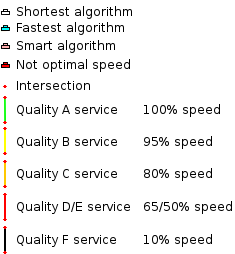
\includegraphics[scale=0.8]{images/legend.png} 
  \caption{Legend of the system}
  \label{legend}
\end{figure}

\begin{table}
\begin{tabularx}{\textwidth}{|c|X|}
\hline 
\textbf{Service level} & \textbf{Description} \\ 
\hline 
A & Free circulation, freedom of movement, high speed \\ 
\hline 
B & Free circulation, less freedom of choosing track, maximum speed starts to be affected \\ 
\hline 
C & Still stable circulation, now choosing the desired track is more of an imposition of the traffic than the willingness of the driver, slower speed \\ 
\hline 
D & Instability, there is no freedom of choosing track, difficult keeping the same speed all the time \\ 
\hline 
E & Instability, circulation starts to stop for brief periods, speed no faster than 50km/h \\ 
\hline 
F & This state represents a traffic jam \\ 
\hline 
\end{tabularx}
\caption{Service levels}
\label{serviceLevels}
\end{table}

\section{Graphical user interface}

When running a simulation in the MAS, it is helpful to have immediate feedback. As can be seen in the Figure \ref{gui}, a real time map of the traffic is depicted. Figure \ref{legend}, as mentioned before, shows an easily readable legend. Depending on which algorithm the agent is using, it is drawn with different colors, the same kind of feedback is obtained from the service level of the segments, they change their color to reflect their status.

The GUI also displays a clock in the upper right corner, that is the time \textit{inside} the simulator, which in combination with the scrollpanel just bellow it that displays what is happening, allows the researcher to keep track of all the events at any point of the simulation.

The last element of the GUI is a slider situated on the bottom right part, that allows the user to change the length between ticks (one tick represents one second inside the simulation), so special cases can be better studied.

\begin{figure}[!ht]
  \centering
  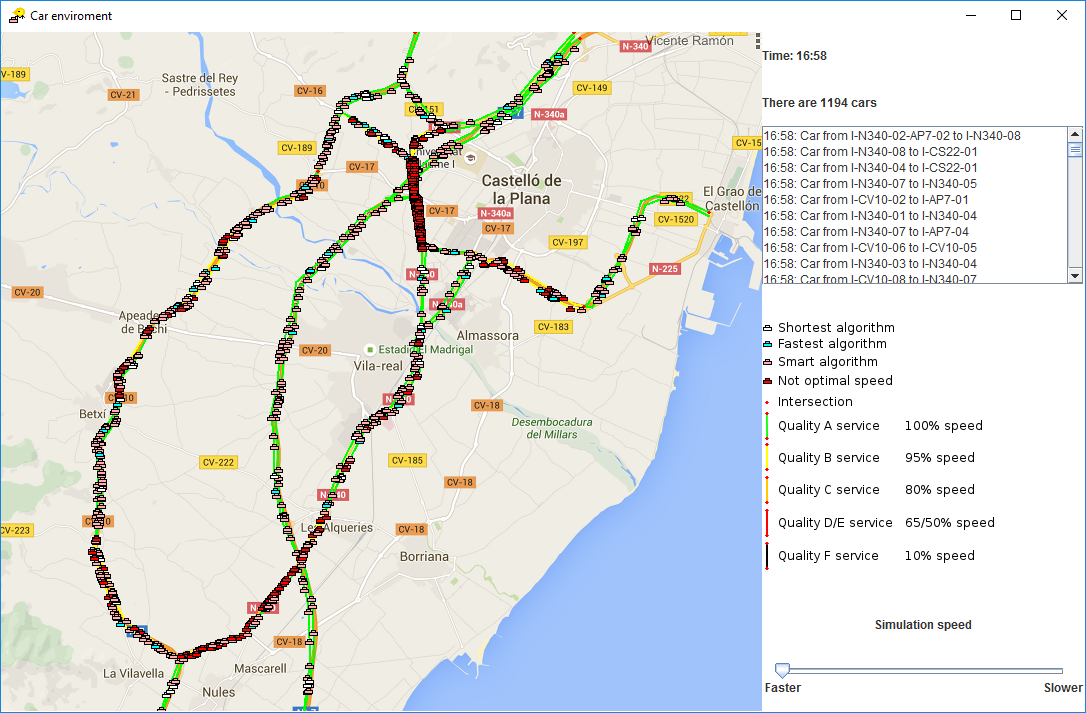
\includegraphics[scale=0.5]{images/gui.png} 
  \caption{Graphical user interface}
  \label{gui}
\end{figure}

























